\documentclass{article}
\usepackage{graphicx}
\usepackage{pdflscape}
\usepackage{lmodern}
\usepackage[T1]{fontenc}
\usepackage{textcomp}
\usepackage{underscore}
\usepackage{listofitems}
\usepackage{hyperref}
\graphicspath{./}

\newcommand{\schema}[2]{#1(#2)}
\newcommand{\pkey}[1]{%
  \setsepchar{,}%
  \readlist*\pkeylist{#1}%
  \foreachitem\x\in\pkeylist[]{\ifnum\xcnt=1\else, \fi\underline{\x}}%
}
\newcommand{\fkey}[1]{%
  \setsepchar{,}%
  \readlist*\fkeylist{#1}%
  \foreachitem\x\in\fkeylist[]{\ifnum\xcnt=1\else, \fi\textit{\x}}%
}

\newcommand{\trightarrow}{\(\rightarrow\)}

\title{COMP3005 Project Design Document}
\author{Steven Pham (101 104 297)}

\begin{document}
\maketitle

\section{Foreword}
I decided to make my implementation as a full webserver/website implementation (which I regret a little) and used Rust as my implementation language for its emphasis on correctness and its powerful type system (which eases a lot of concerns with the loosely typed nature of the web).

The github for the project is \href{https://github.com/Eliasin/lookInnaBook}{here} (https://github.com/Eliasin/lookInnaBook). I have also deployed it to a DigitalOcean droplet for you to try out \href{http://owncloud.eliasin.ca:8000/}{here} (http://owncloud.eliasin.ca:8000/).

You can create your own account on the deployment or use one that I've used for testing, its credentials are ``test2@local'' as the email and ``123'' as the password. Similarly, an admin account I've used for testing has the credentials ``admin2@local'' and ``123''.

A funny thing that happened is that I ended up finding a bug in the open source plotting library \href{https://lib.rs/crates/poloto}{poloto} where it would not escape ampersands and other HTML characters in the generated SVGs (would break when a publisher had \& in its name).

\section{ER Diagram}
The ER diagram is shown on the next page in landscape format.
Some assumptions made are:
\begin{itemize}
  \item We only offer services to Canadian customers.
  \item Payment can be processed with only the card number, expiry, CVV (number on back), and the cardholder name
  \item Each order can only ship to one address
  \item Each book can be uniquely identified by an ISBN
  \item A credit card number does not uniquely identify a method of payment (I did some cursory research and apparently sometimes these are reused with different CVV numbers)
  \item A publisher's payment information can be summed up in a bank number
  \item A book collection can only be curated by one owner at a time
  \item A book's data can never be completely removed from the database as this would mess with previous order information, instead, books are discontinued which prevents purchasing and hides them from the store
  \item If no owner accounts exist, an owner can be bootstrapped by logging into a default owner account with credentials ``admin@local'' and ``123''. This default owner account cannot curate collections and is disabled when another account is created.
  \item All orders and restock orders have the ability database-wise to be set to whatever the state of the order is, but we have no outside triggers to change these so they will always be stuck as PENDING or PR (processing)
  \item The restock orders will order the previous month's sales including the sale that triggered the restock
\end{itemize}

\begin{landscape}
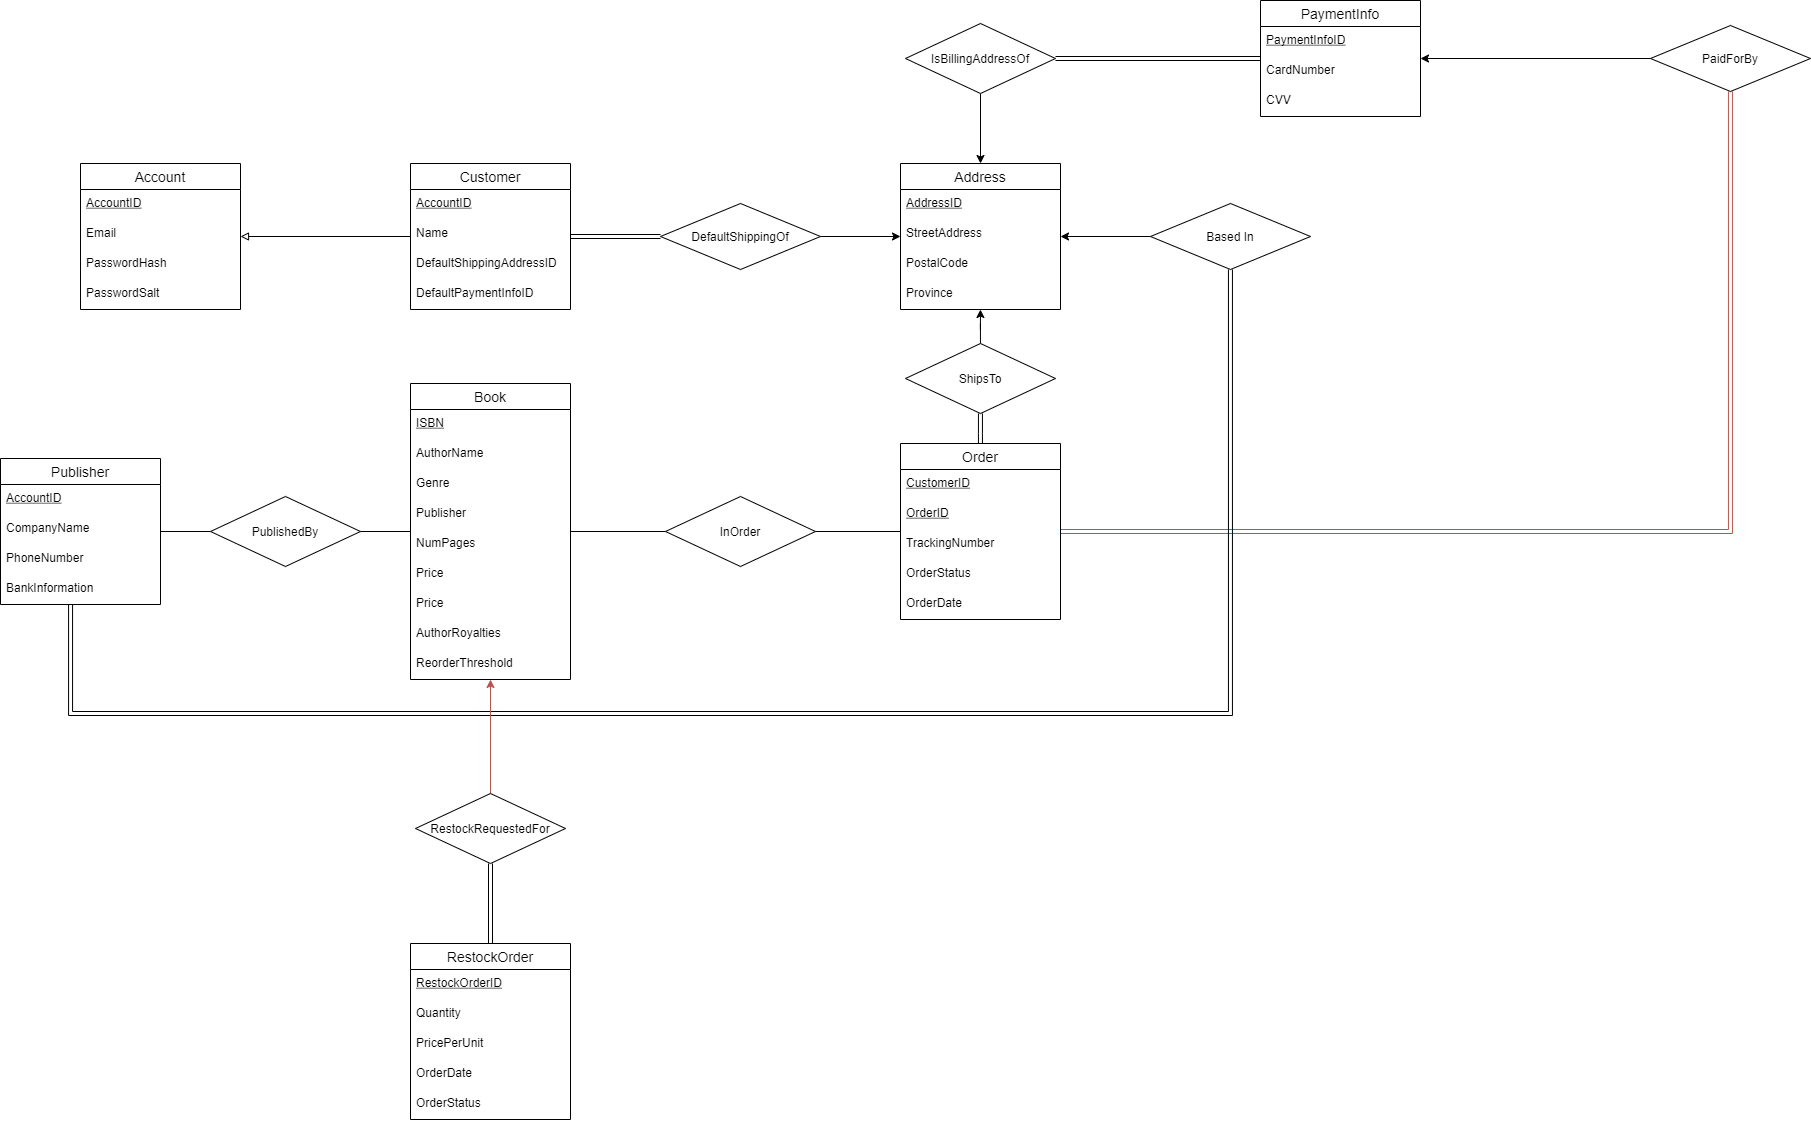
\includegraphics[height=\textwidth]{er}
\end{landscape}

\section{Relations Schema}
The above ER diagram can be broken down into the relation schema below. Primary keys are denoted by underscores. Foreign keys are denoted in italics.
\begin{itemize}
  \item \schema{book}{\pkey{isbn}, title, author_name, genre, publisher, num_pages, price, author_royalties, reorder_threshold, stock, discontinued, \fkey{publisher_id}}
  \item \schema{address}{\pkey{address_id}, street_address, postal_code, province}
  \item \schema{customer}{\pkey{customer_id}, name, email, password_hash, password_salt, \fkey{default_shipping_address_id, default_payment_info_id}}
  \item \schema{payment_info}{\pkey{payment_info_id}, name_on_card, expiry, card_number, cvv, \fkey{billing_address}}
  \item \schema{publisher}{\pkey{publisher_id}, company_name, phone_number, bank_number, \fkey{address_id}}
  \item \schema{order}{\pkey{order_id}, \fkey{customer_id, shipping_address}, tracking_number, order_status, order_date, \fkey{payment_info_id}}
  \item \schema{in_order}{\fkey{\pkey{isbn, order_id}}, quantity}
  \item \schema{restock_order}{\pkey{restock_order_id}, \fkey{isbn}, quantity, price_per_unit, order_date, order_status}
  \item \schema{in_cart}{\fkey{\pkey{isbn, customer_id}}, quantity}
  \item \schema{owner}{\pkey{owner_id}, name, email, password_hash, password_salt}
  \item \schema{book_collection}{\pkey{collection_id}, \fkey{curator_owner_id}, name}
  \item \schema{in_collection}{\fkey{\pkey{collection_id, isbn}}}
\end{itemize}

\section{Functional Dependencies}
Below are the functional dependencies for this domain.
\begin{itemize}
  \item ISBN \trightarrow{} Title, AuthorName, Genre, Publisher, NumPages, Price, AuthorRoyalties, ReorderThreshold, Stock, Discontinued
  \item AddressID \trightarrow{} StreetAddress, PostalCode, Province
  \item CustomerID \trightarrow{} CustomerName, CustomerEmail, CustomerPasswordHash, CustomerPasswordSalt, DefaultShippingAddressID, DefaultPaymentInfoID
  \item Email \trightarrow{} CustomerID, CustomerName, CustomerPasswordHash, CustomerPasswordSalt, DefaultShippingAddressID, DefaultPaymentInfoID
  \item PaymentInfoID \trightarrow{} NameOnCard, ExpiryDate, CardNumber, CVV, BillingAddressID
  \item PublisherID \trightarrow{} CompanyName, PhoneNumber, BankNumber, AddressID
  \item OrderID \trightarrow{} CustomerID, TrackingNum, OrderStatus, OrderDate, ShippingAddressID, PaymentInfoID
  \item OrderID, BookISBN \trightarrow{} OrderQuantity
  \item CustomerID, BookISBN \trightarrow{} CartQuantity
  \item RestockOrderID \trightarrow{} BookISBN, Quantity, PricePerUnit, OrderDate, OrderStatus
  \item OwnerID \trightarrow{} OwnerName, OwnerEmail, OwnerPasswordHash, OwnerPasswordSalt
  \item BookCollectionID \trightarrow{} OwnerID, Name
\end{itemize}

\section{Testing For Good Form}
We will now test to make sure that all of our relations are in good form. We will test that each relation is in 3NF.
\subsection{Book}
Functional dependencies:
\begin{itemize}
  \item ISBN \trightarrow{} Title, AuthorName, Genre, Publisher, NumPages, Price, AuthorRoyalties, ReorderThreshold
\end{itemize}

ISBN is trivially a super key so this relation is in BCNF.

\subsection{AddressID}
Functional dependencies:
\begin{itemize}
  \item AddressID \trightarrow{} StreetAddress, PostalCode, Province
\end{itemize}

AddressID is trivially a super key for address.

\subsection{Customer}
\begin{itemize}
  \item CustomerID \trightarrow{} CustomerName, CustomerEmail, CustomerPasswordHash, CustomerPasswordSalt, DefaultShippingAddressID, DefaultPaymentInfoID
  \item CustomerEmail \trightarrow{} CustomerID, CustomerName, CustomerPasswordHash, CustomerPasswordSalt, DefaultShippingAddressID, DefaultPaymentInfoID
\end{itemize}

Both CustomerID and CustomerEmail are trivially superkeys.

\subsection{PaymentInfo, Publisher, Order, RestockOrder, Owner, BookCollection}
All of these relations are also 3NF in a similar way where there is only one functional dependency which is some ID attribute to the rest of the relation.

\subsection{InOrder}
Functional dependencies:
\begin{itemize}
  \item OrderID, BookISBN \trightarrow{} OrderQuantity
\end{itemize}

(OrderID, BookISBN) is trivially the super key since it determines the other attribute in the relation.

\subsection{InCart}
Functional dependencies:
\begin{itemize}
  \item CustomerID, BookISBN \trightarrow{} CartQuantity
\end{itemize}

(CustomerID, BookISBN) is trivially the super key since it determines the other attribute in the relation.

All of our relations are in good form.

\section{Schema Diagram}

\begin{landscape}
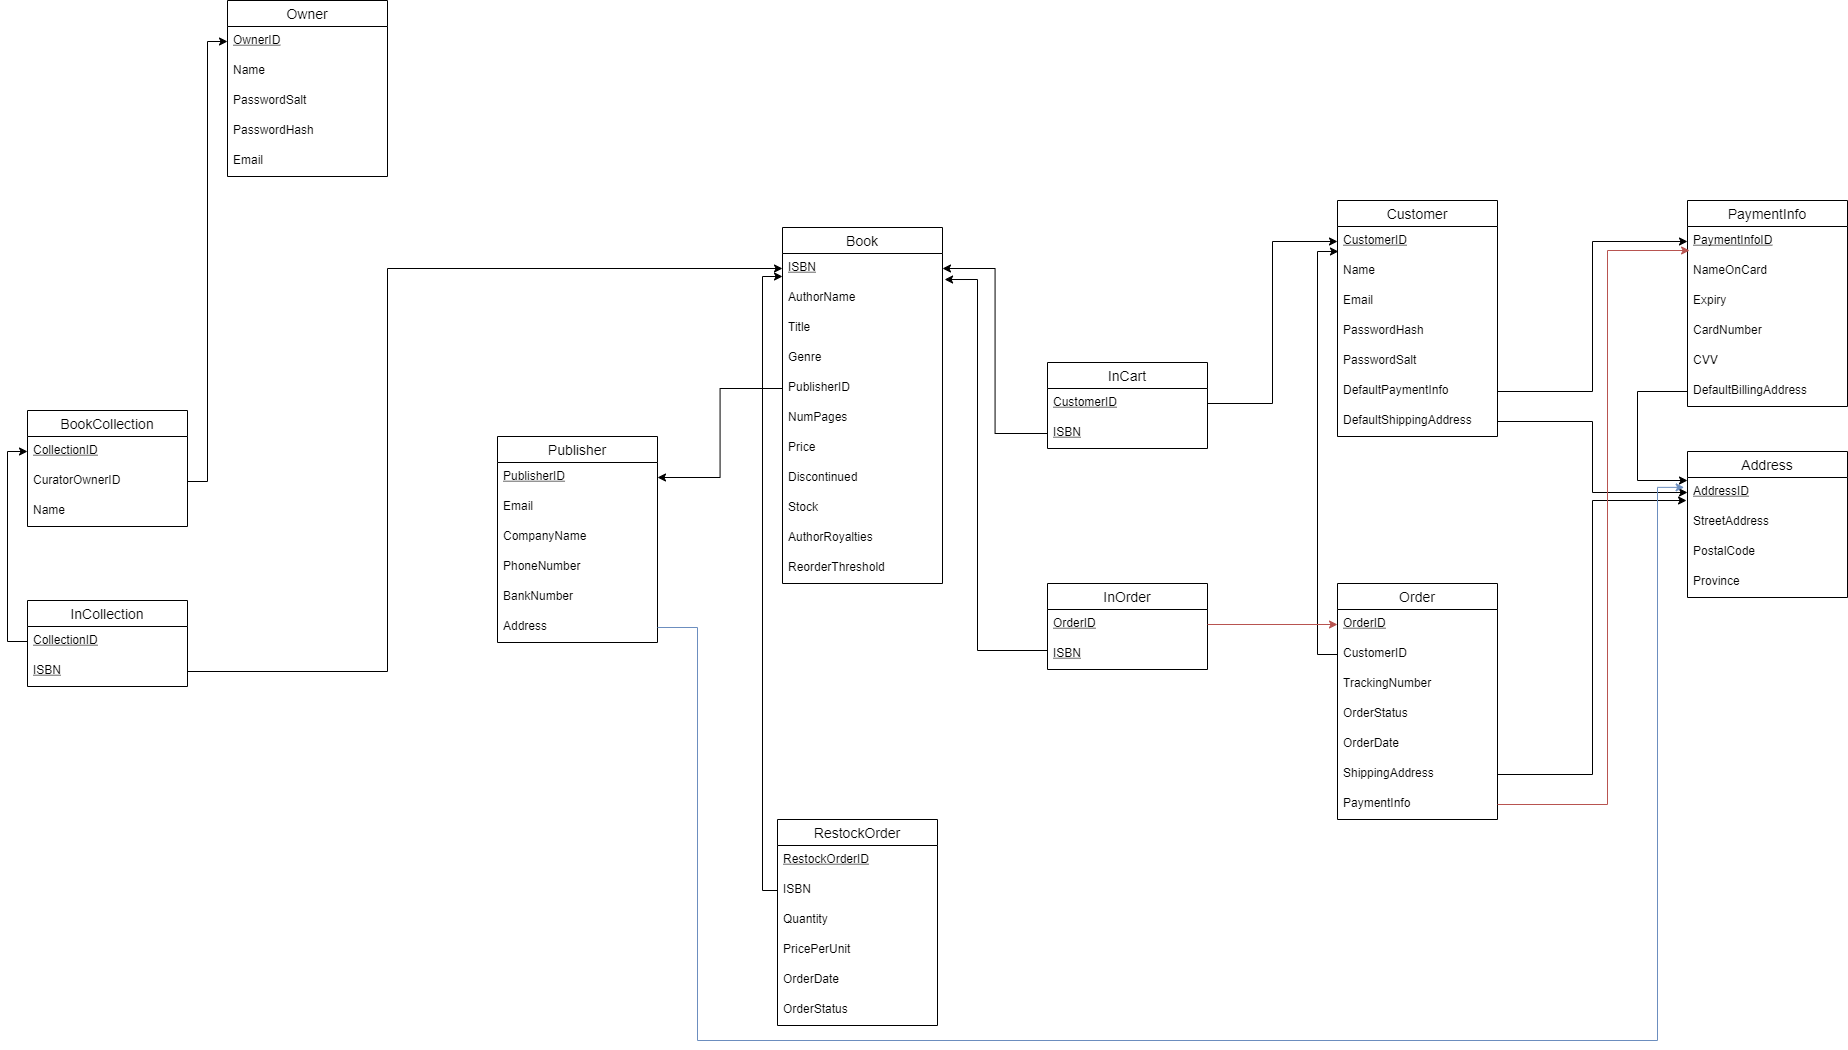
\includegraphics[height=\textwidth]{schema}
\end{landscape}

\section{Implementation}
The general architecture of the application is divided at the file level. The main.rs file mostly does some library setup, the endpoint.rs file defines all of the HTTP endpoints the application exposes, the db.rs file exposes operations and queries on the database that are used by the endpoints, the schema.rs file exposes structures that represent database entities.

Below I will go over a select number of use cases in terms of control flow.

Loading site main page:
\begin{enumerate}
  \item Client makes HTTP request to server for index
  \item Server matches path to registered routes (defined in main.rs)
  \item Matching path is found (paths are defined in endpoints.rs)
  \item Index path determines whether or not user is logged in by checking cookies for session tokens
  \item If the user is logged in, it adds information to the HTML rendering context to among other things, display the correct nav bar links (if logged in, no log in link, for example)
  \item Endpoint makes DB query to get all books (no pagination implemented) to populate the main page
  \item Book information is placed in the HTML rendering context
  \item HTML template (index.html.tera under templates/) is rendered
  \item HTTP response is sent to user
\end{enumerate}

Logging in as a customer (note that I did not implement HTTPS so passwords are not encrypted by default):
\begin{enumerate}
  \item Client submits HTML form to log in
  \item Server gets the login information for a given email if it exists
  \item Server checks if the password field of the form hashes to the correct bcrypt hash
  \item If password is correct, a session cookie is added to running memory corresponding to the user and we set the user cookie to the session token
\end{enumerate}

A user tries to login to a page they are not authorized to view:
\begin{enumerate}
  \item Client tries to forge HTTP request to edit/view data
  \item Rocket tries to create Owner type as a request guard to verify that the request comes from someone with owner permissions (implementation is in request_guard.rs)
  \item Request guard looks for owner session token in HTTP request
  \item Implementation does not find one or finds forged token
  \item Token does not correspond to logged in owner, request is denied with 403 HTTP response
\end{enumerate}

A user tries to use default admin session token when owner accounts exist:
\begin{enumerate}
  \item Client tries to view owner protected content
  \item Owner request guard implementation is triggered
  \item Request guard checks if session token exists
  \item Owner session token is identified, we check if any non default owner session tokens exist
  \item If they do not, we now check if there are any owners registered in the database
  \item Owners exist in database, default owner session token is removed and access is denied with 403 HTTP response
\end{enumerate}

A diagram showing the low level control flow of the application is below.

\begin{landscape}
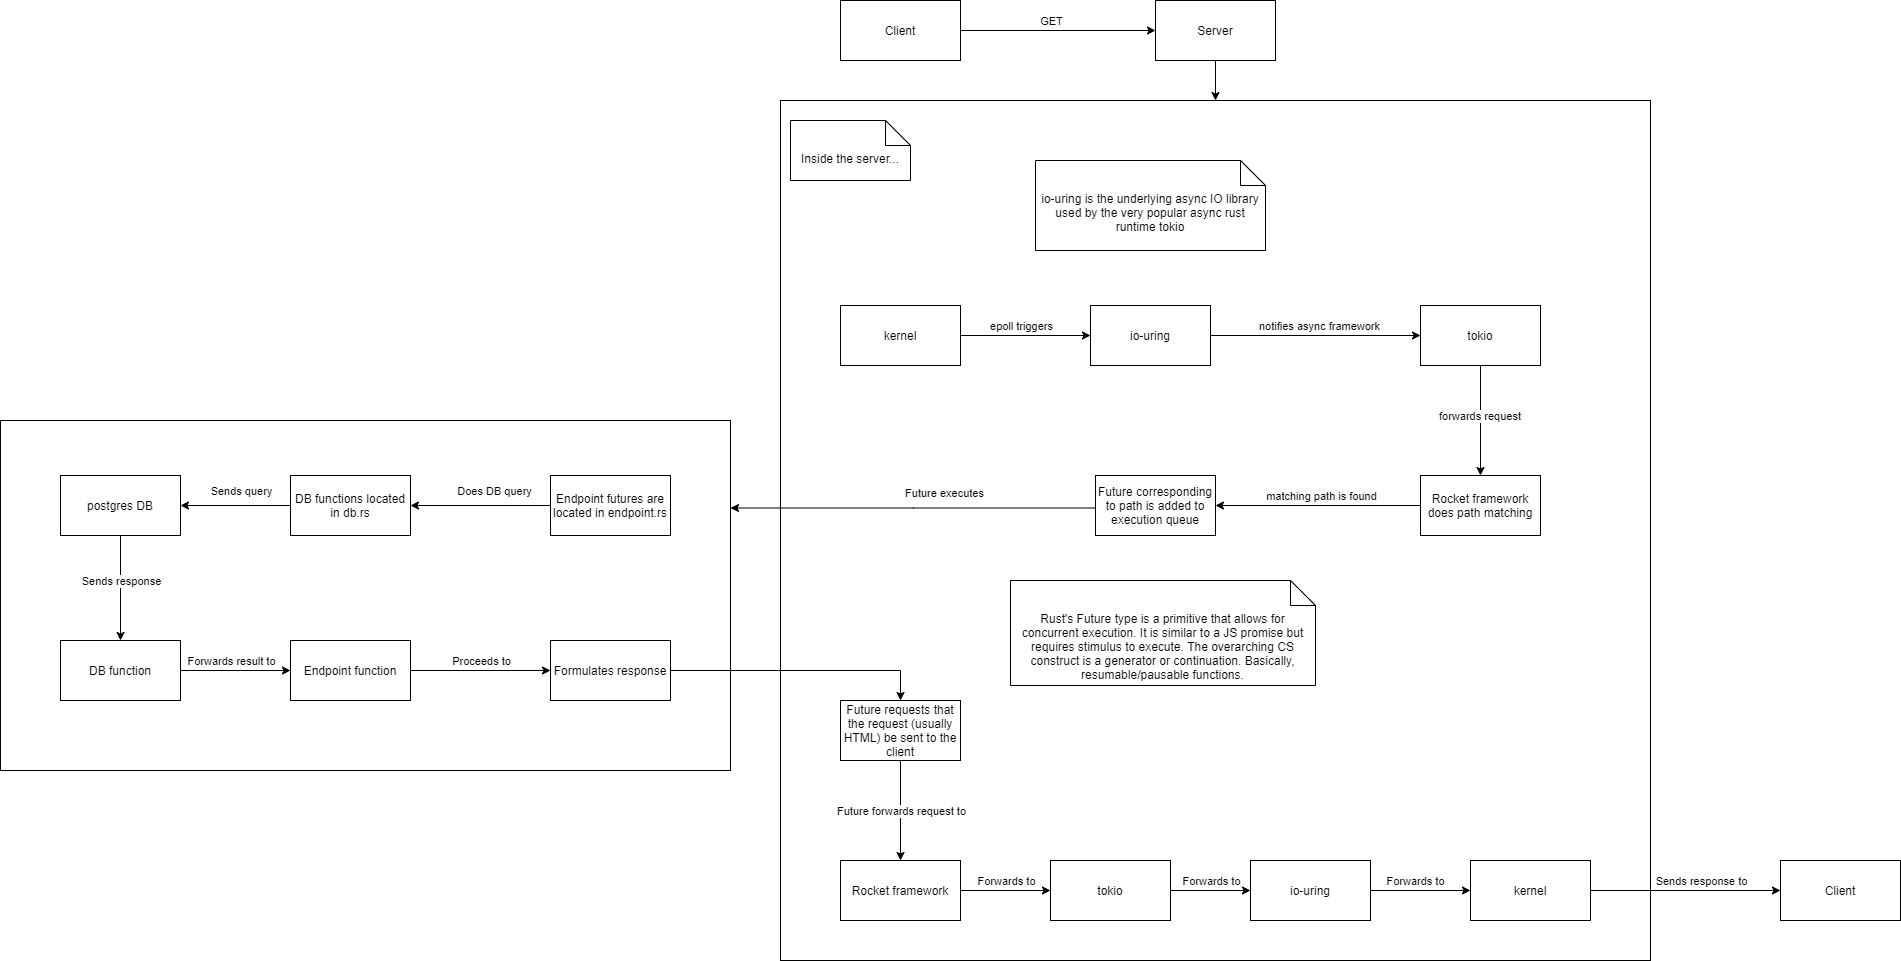
\includegraphics[height=\textwidth]{implementation}
\end{landscape}

Here are some screenshots of the UI (I use a dark-mode browser plugin so it will look different to you.)

\begin{center}
  Home Screen
  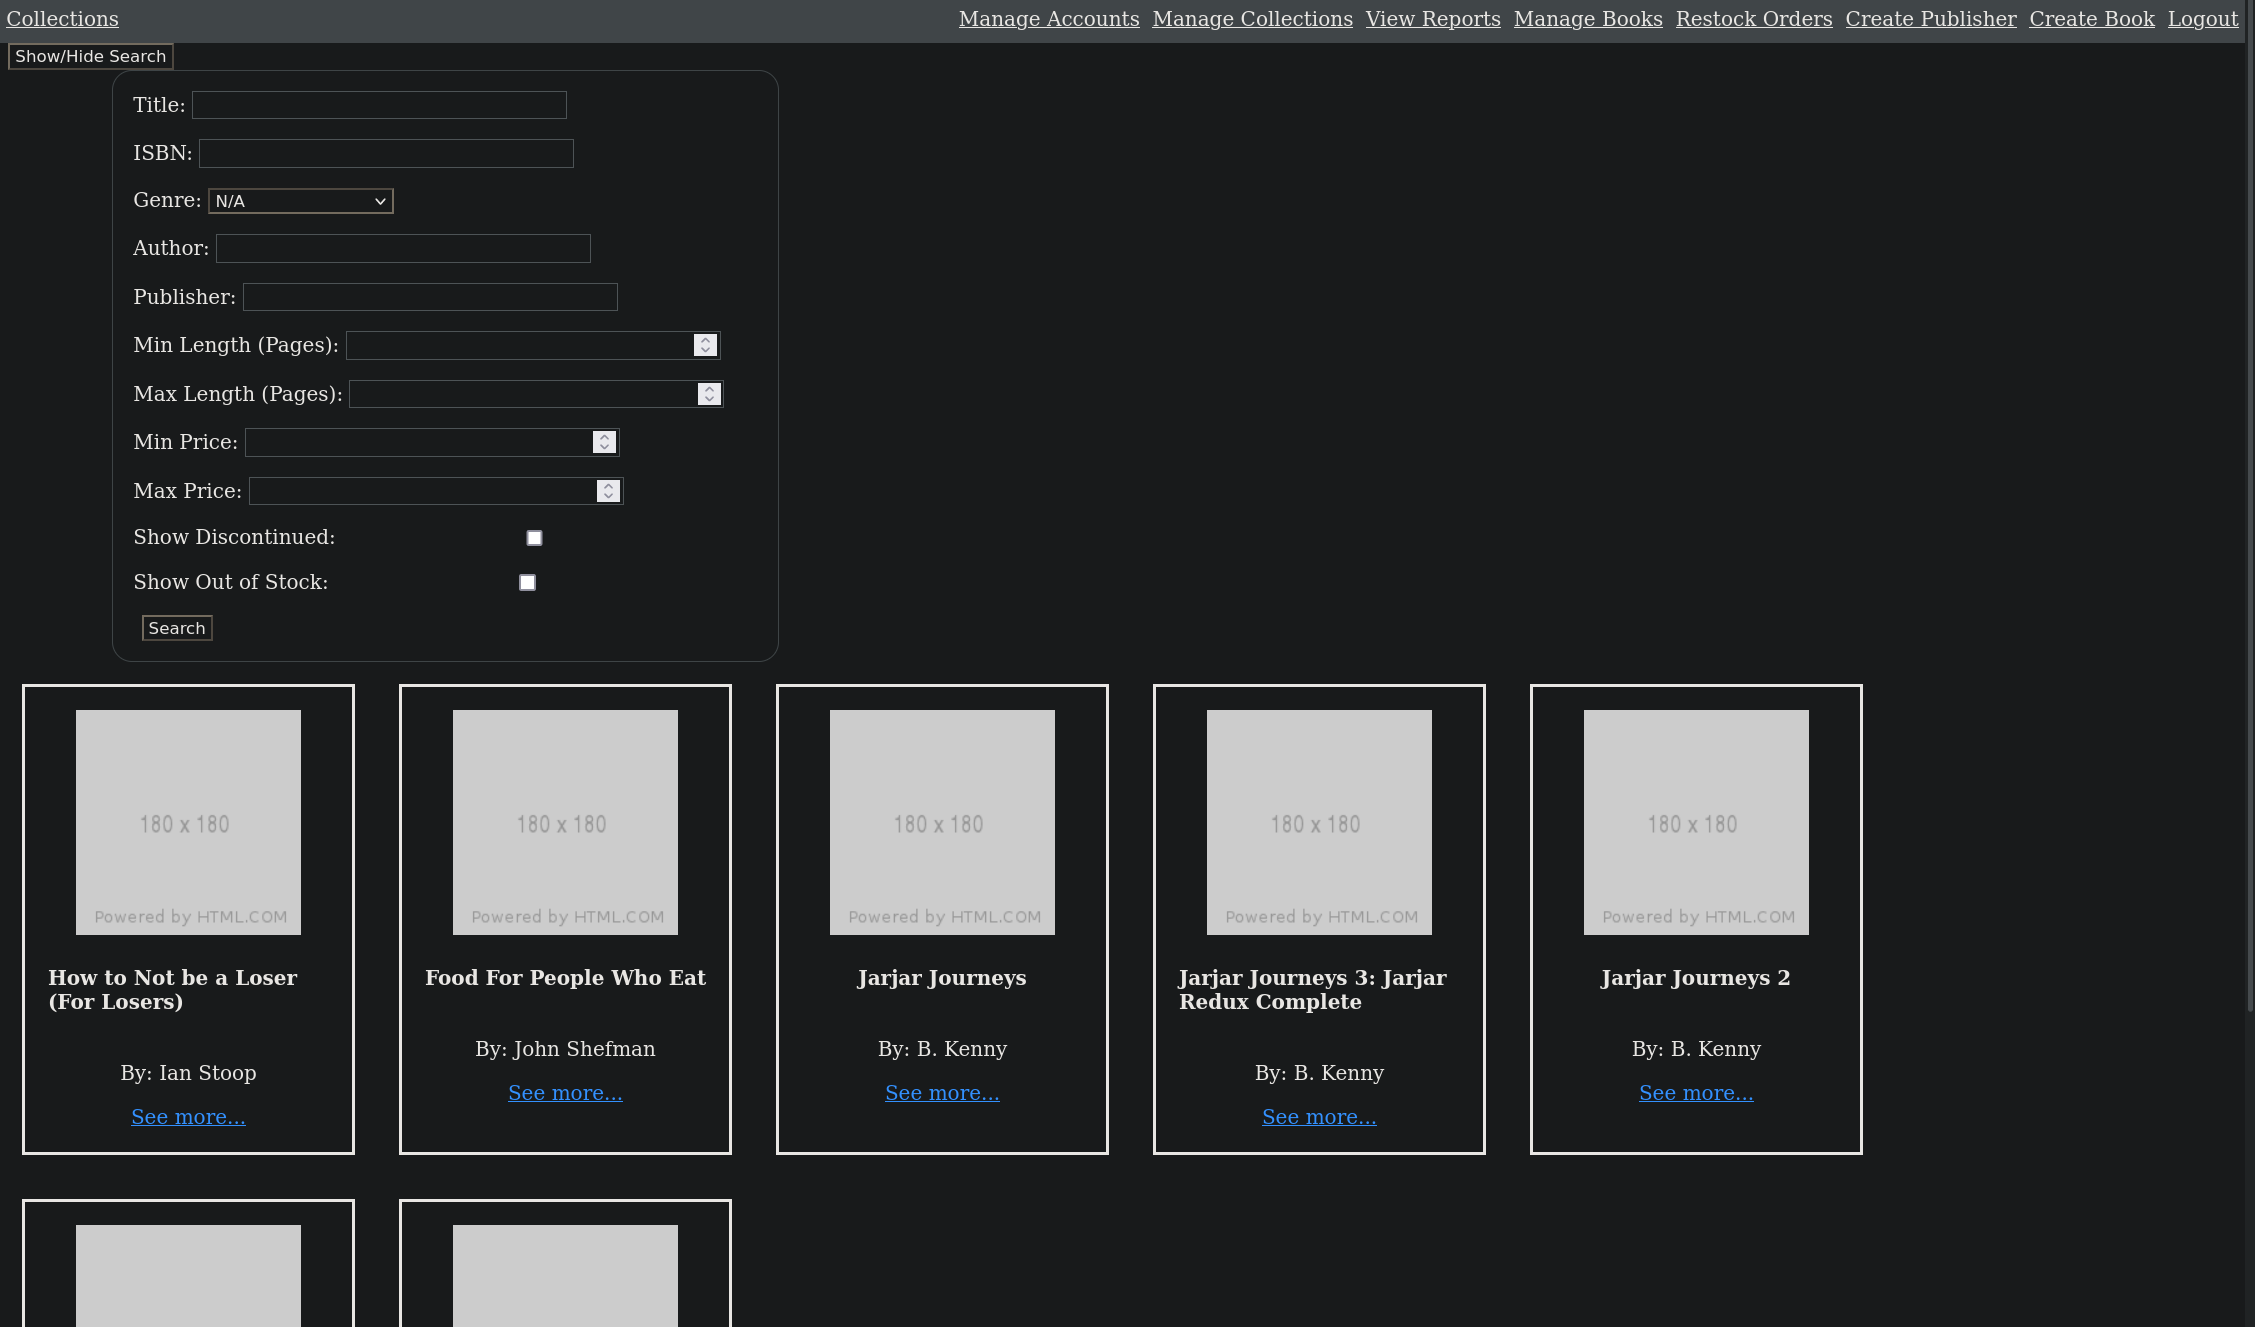
\includegraphics[width=\textwidth]{home_screen}
  Reports
  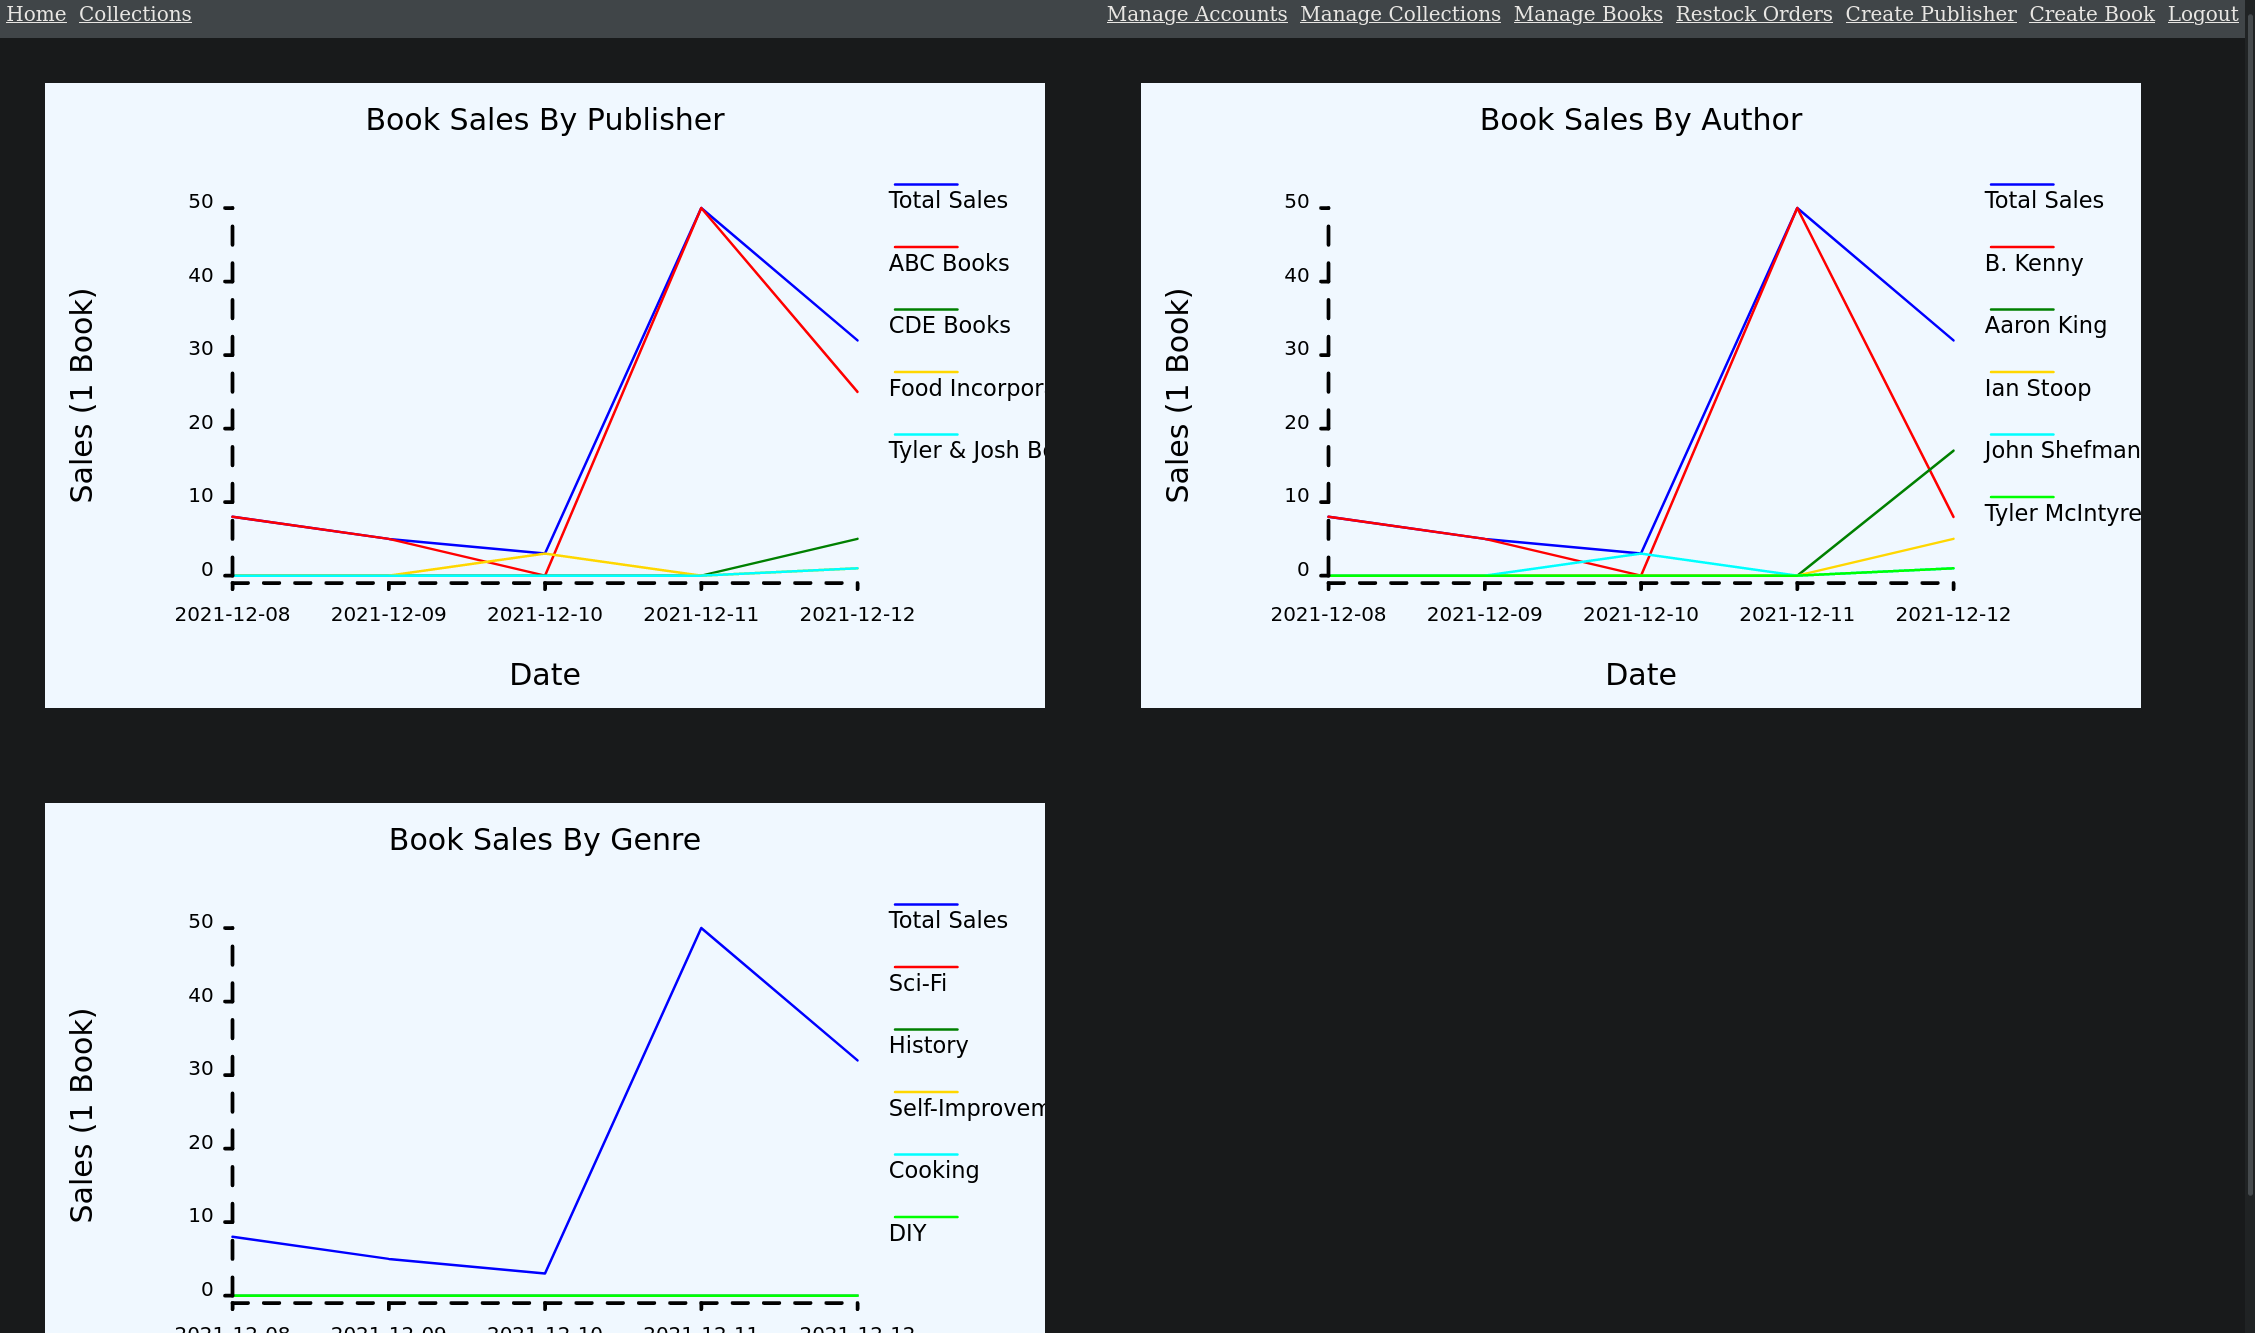
\includegraphics[width=\textwidth]{reports}
  Manage Books
  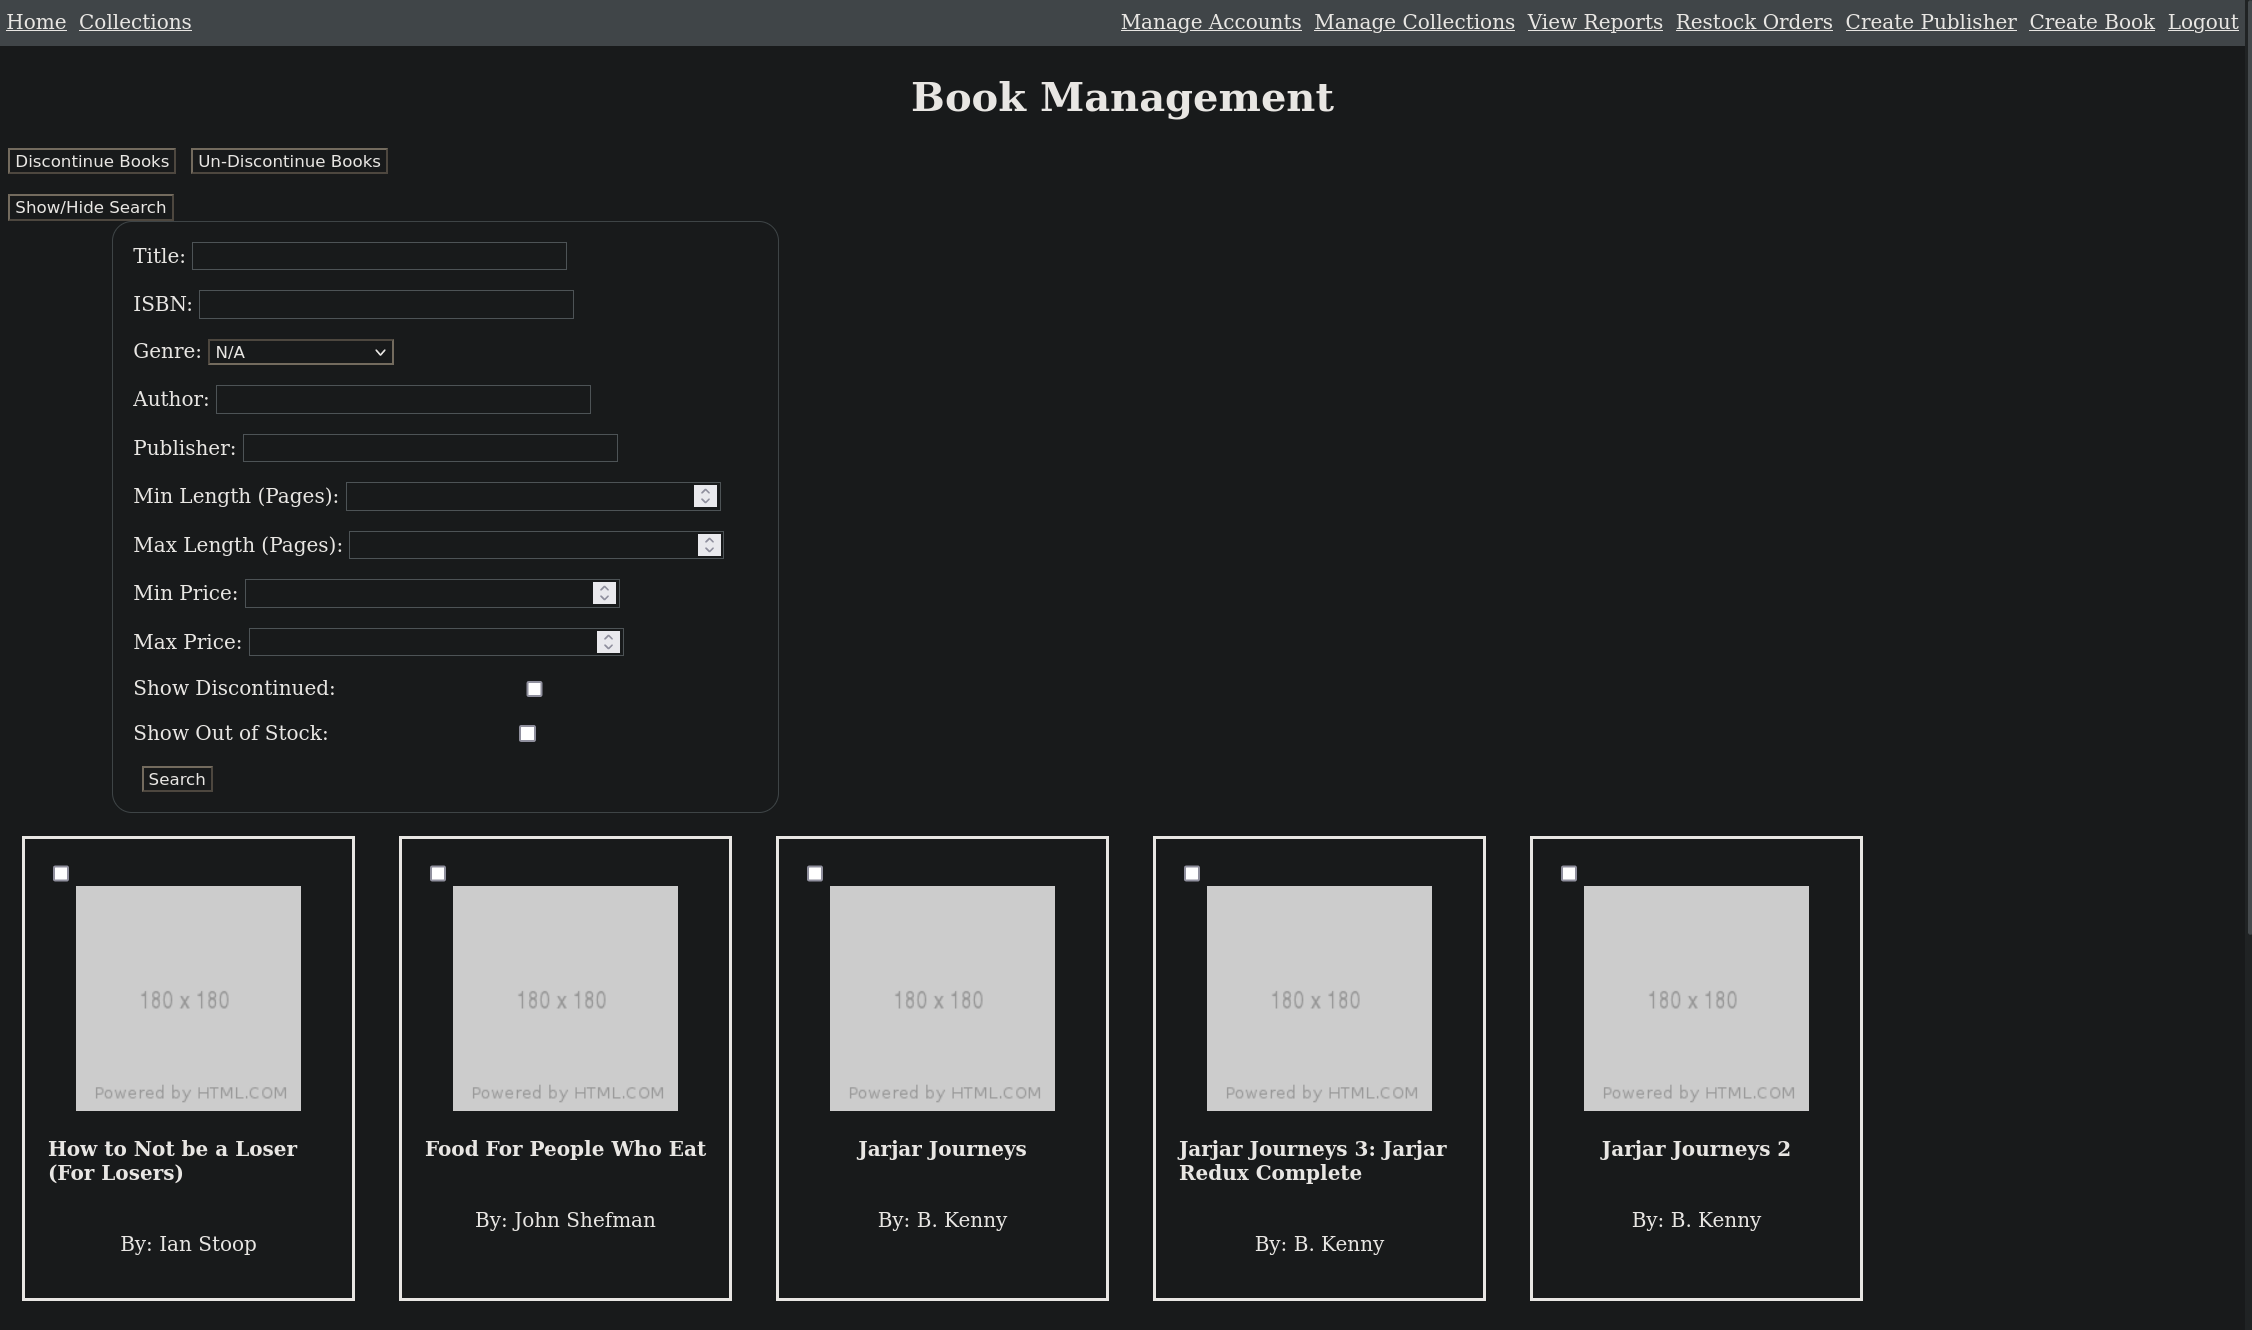
\includegraphics[width=\textwidth]{manage_books}
  Order Details
  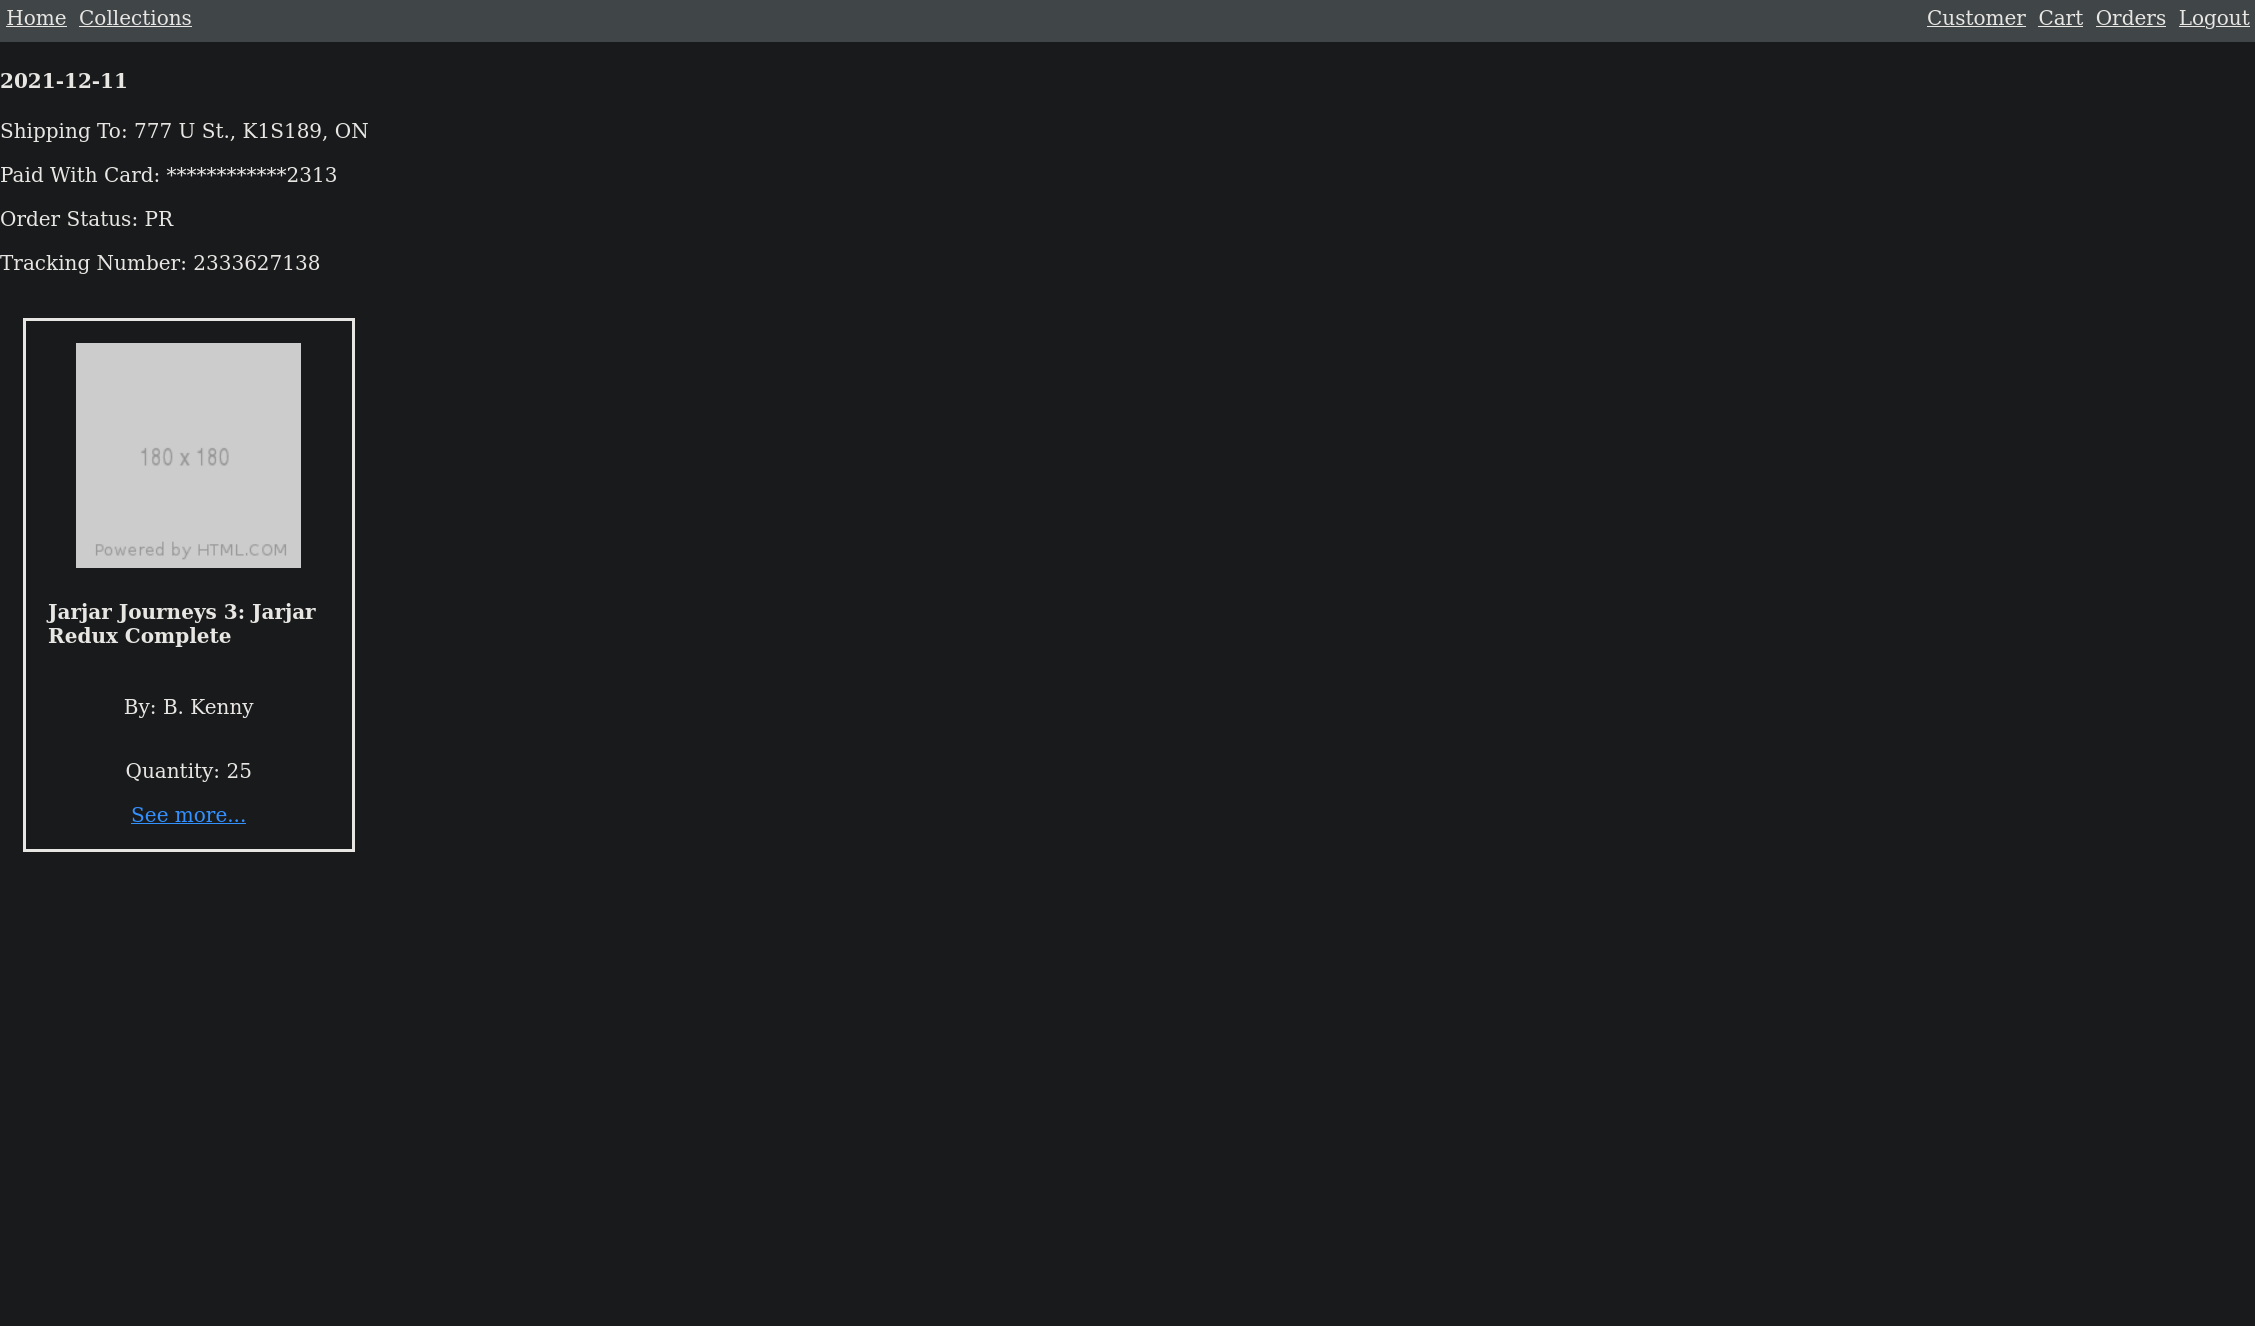
\includegraphics[width=\textwidth]{order}
  Orders
  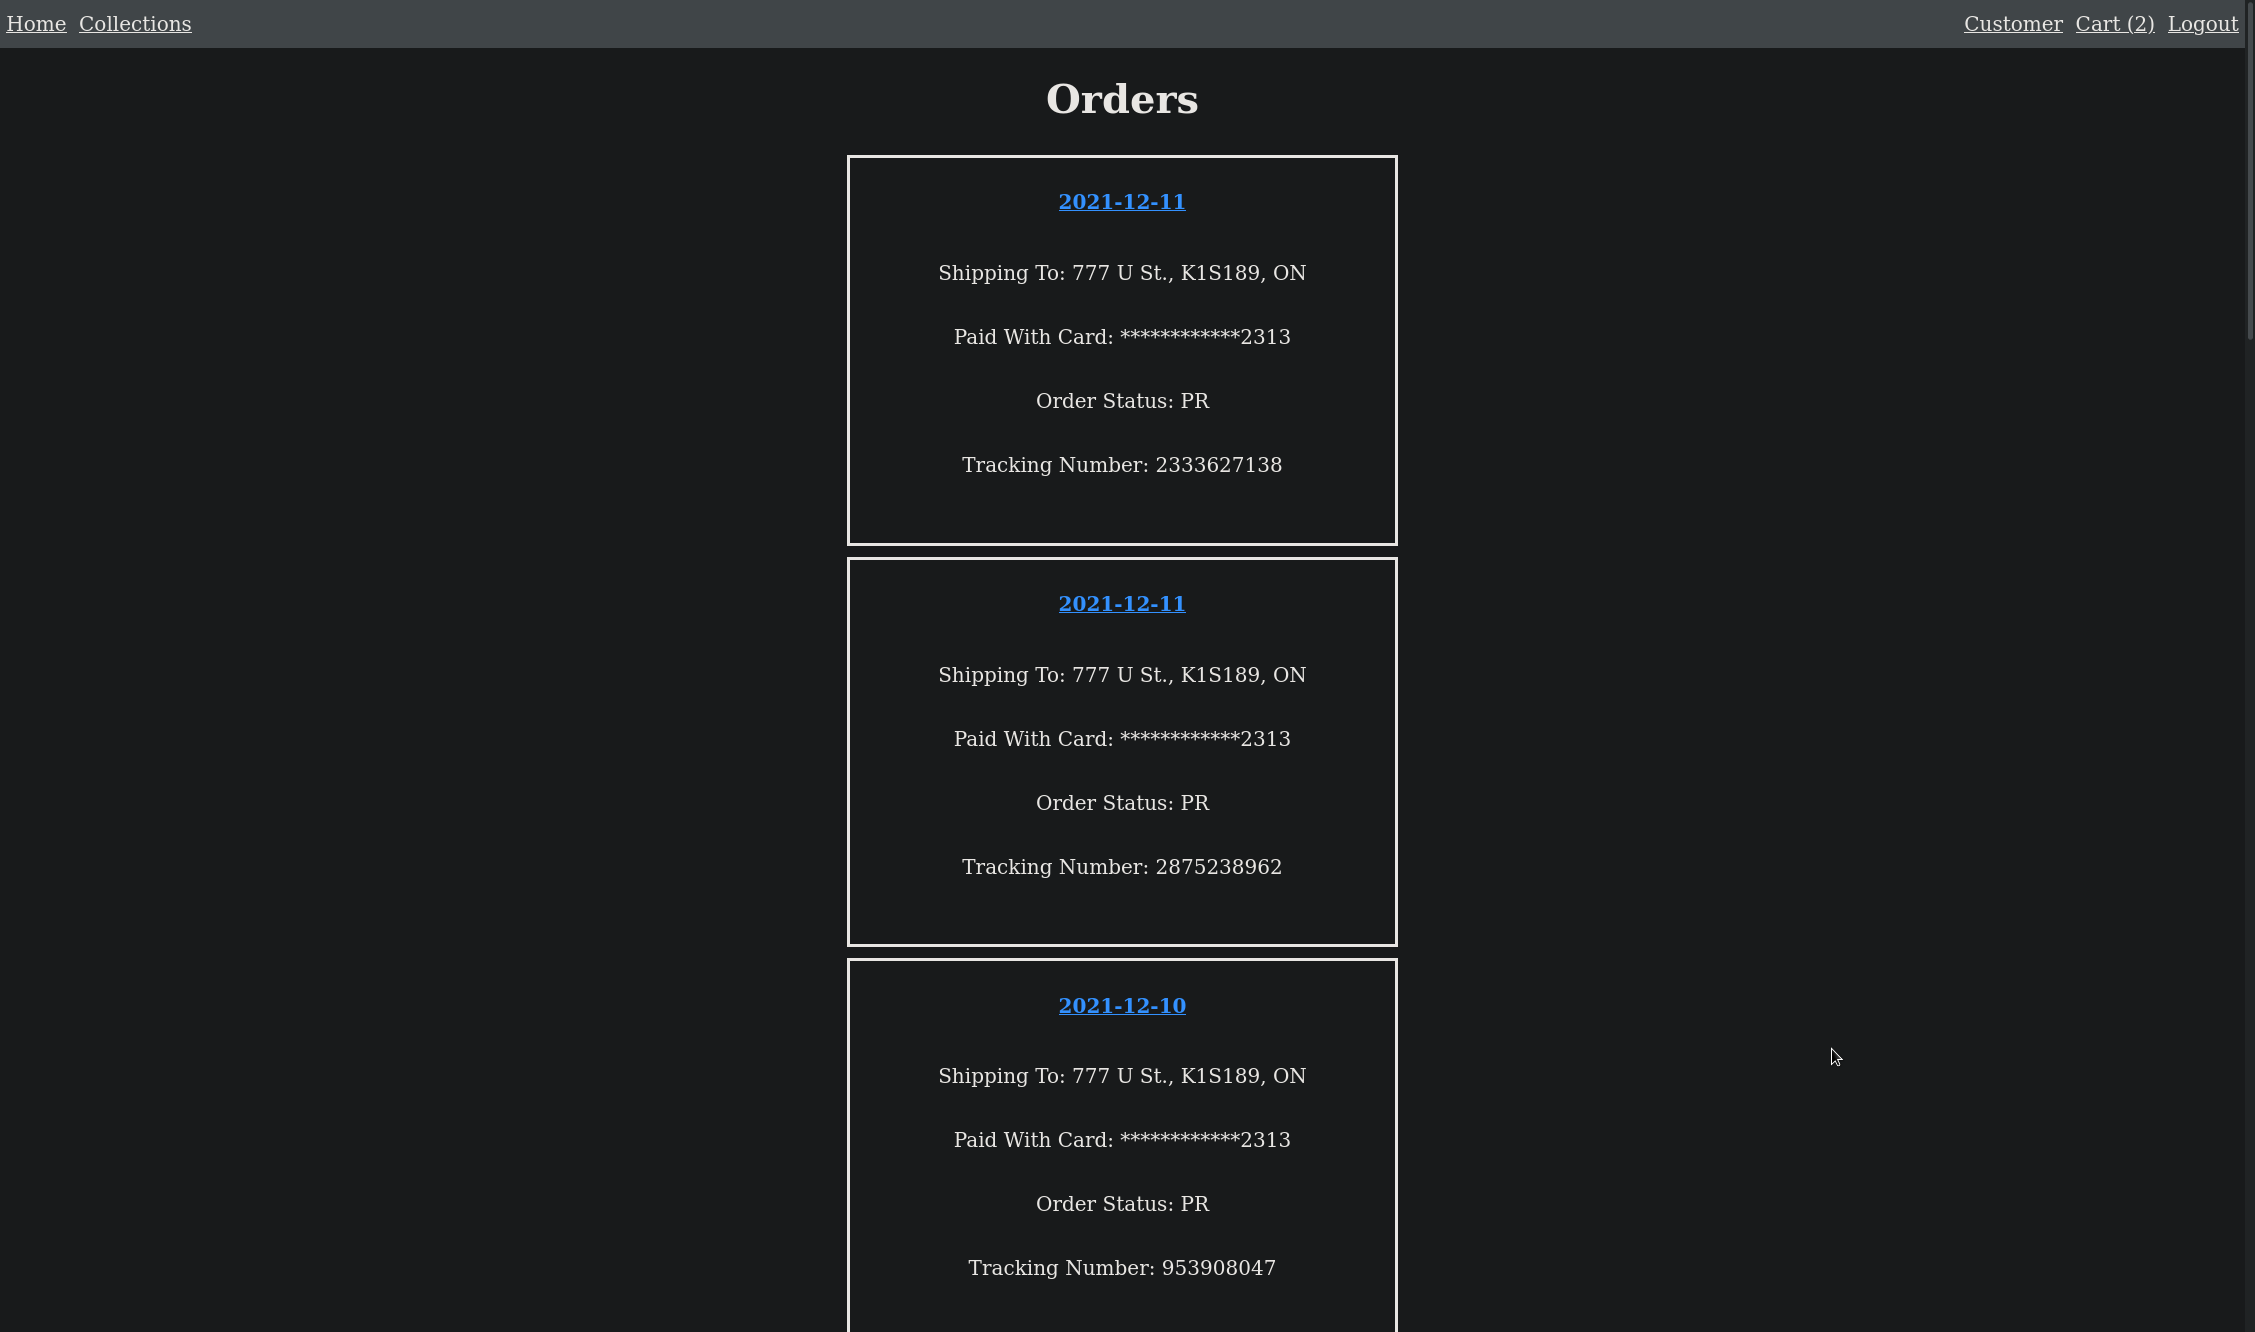
\includegraphics[width=\textwidth]{orders}
  Cart
  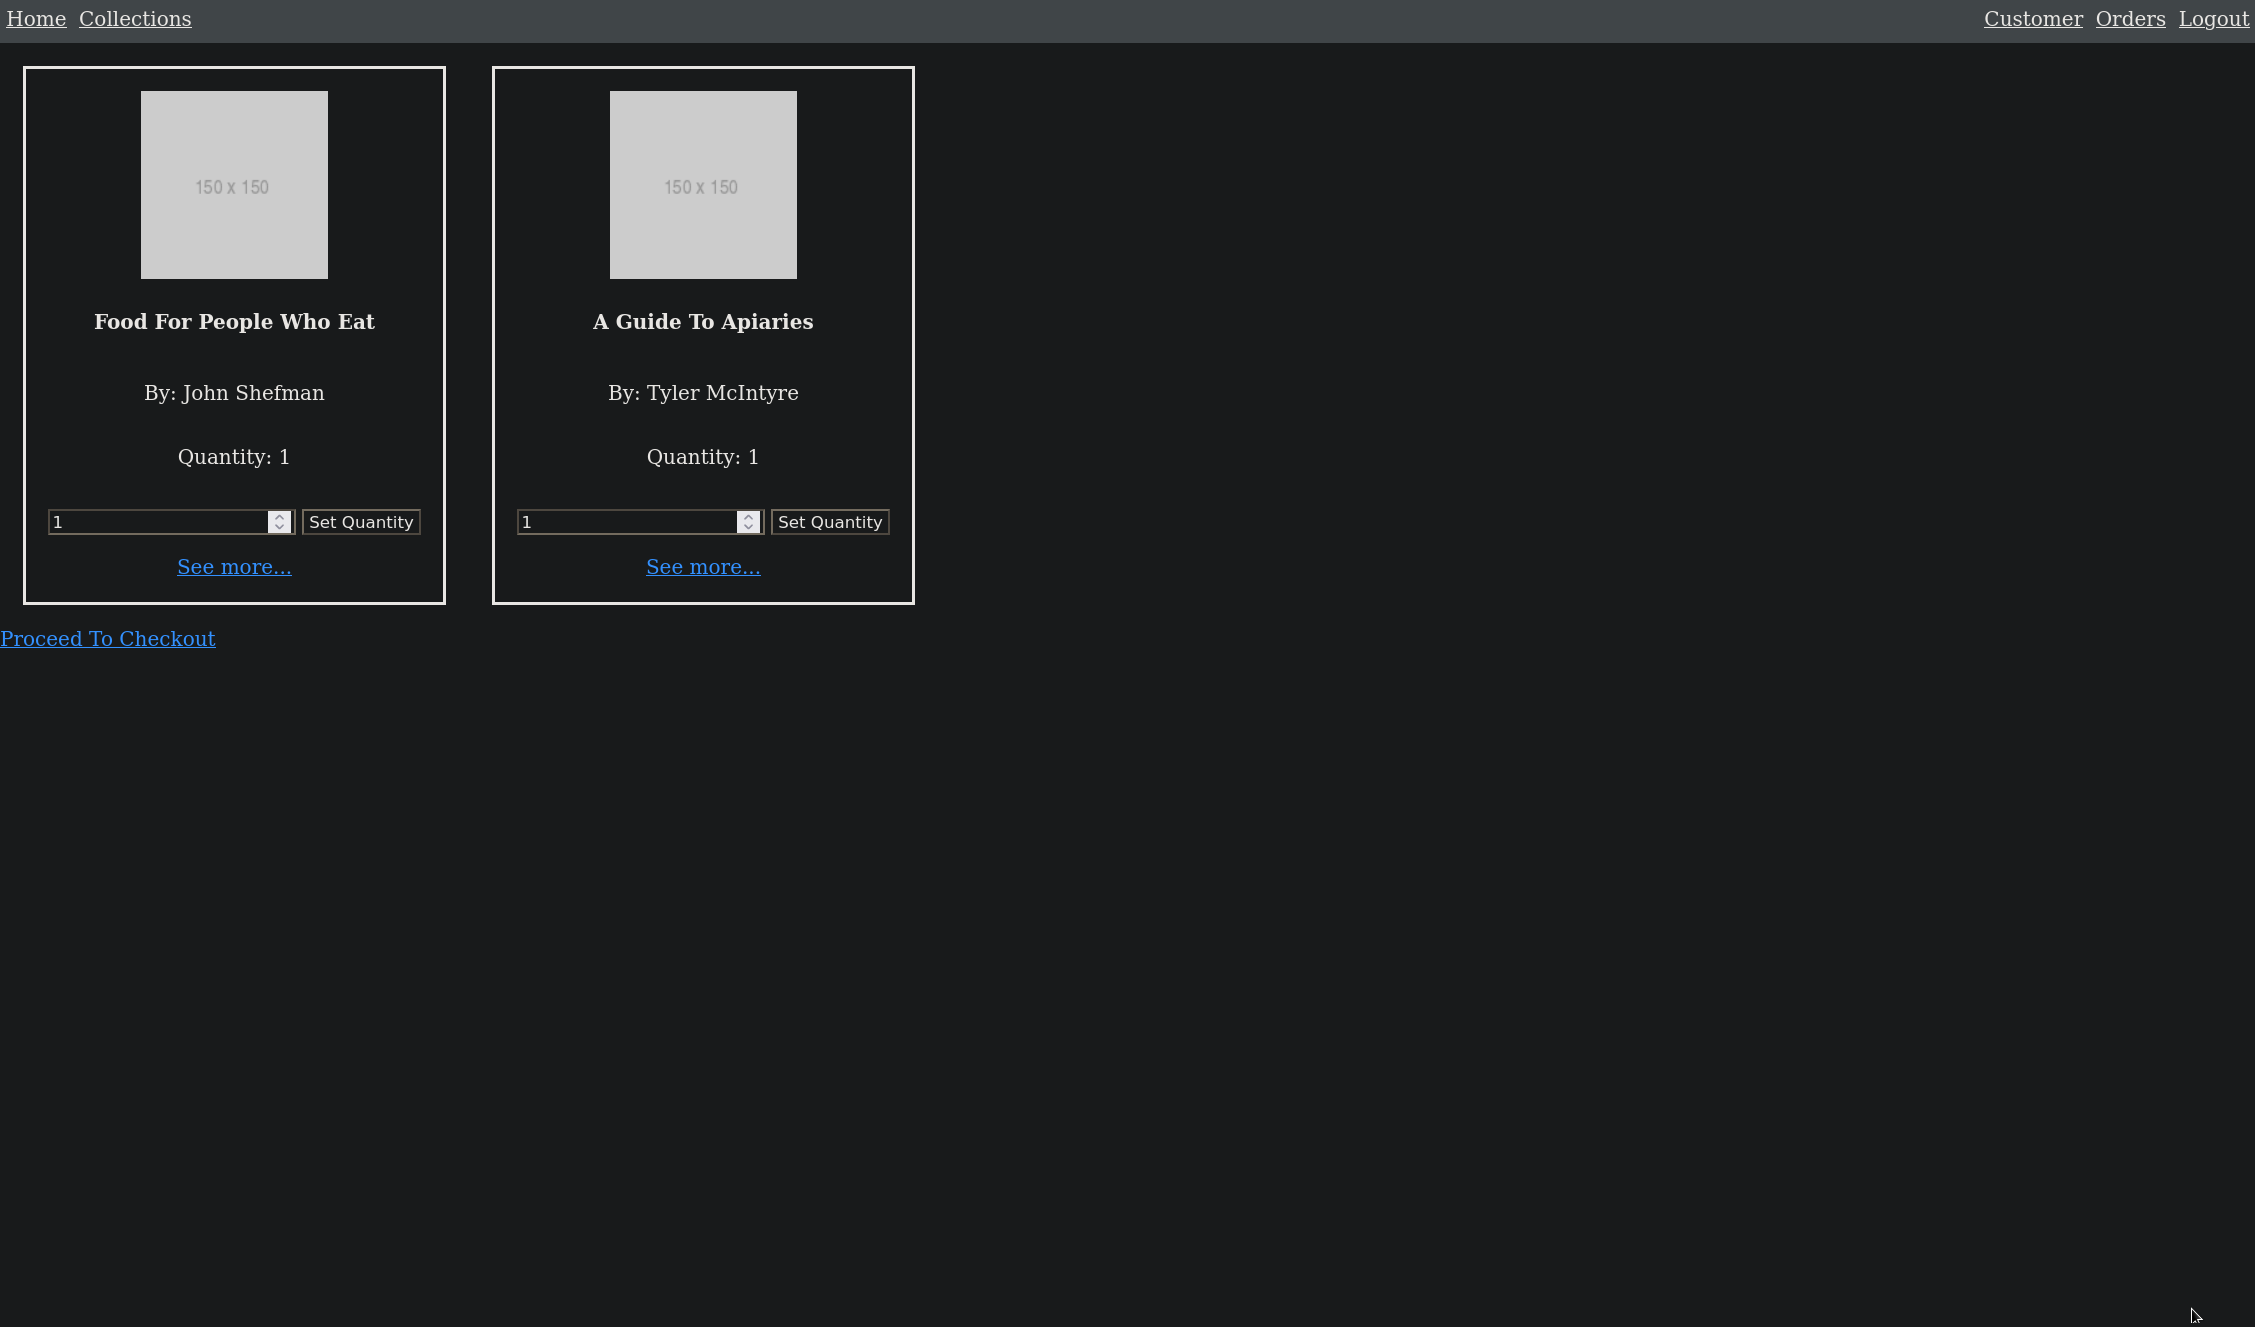
\includegraphics[width=\textwidth]{cart}
  Checkout
  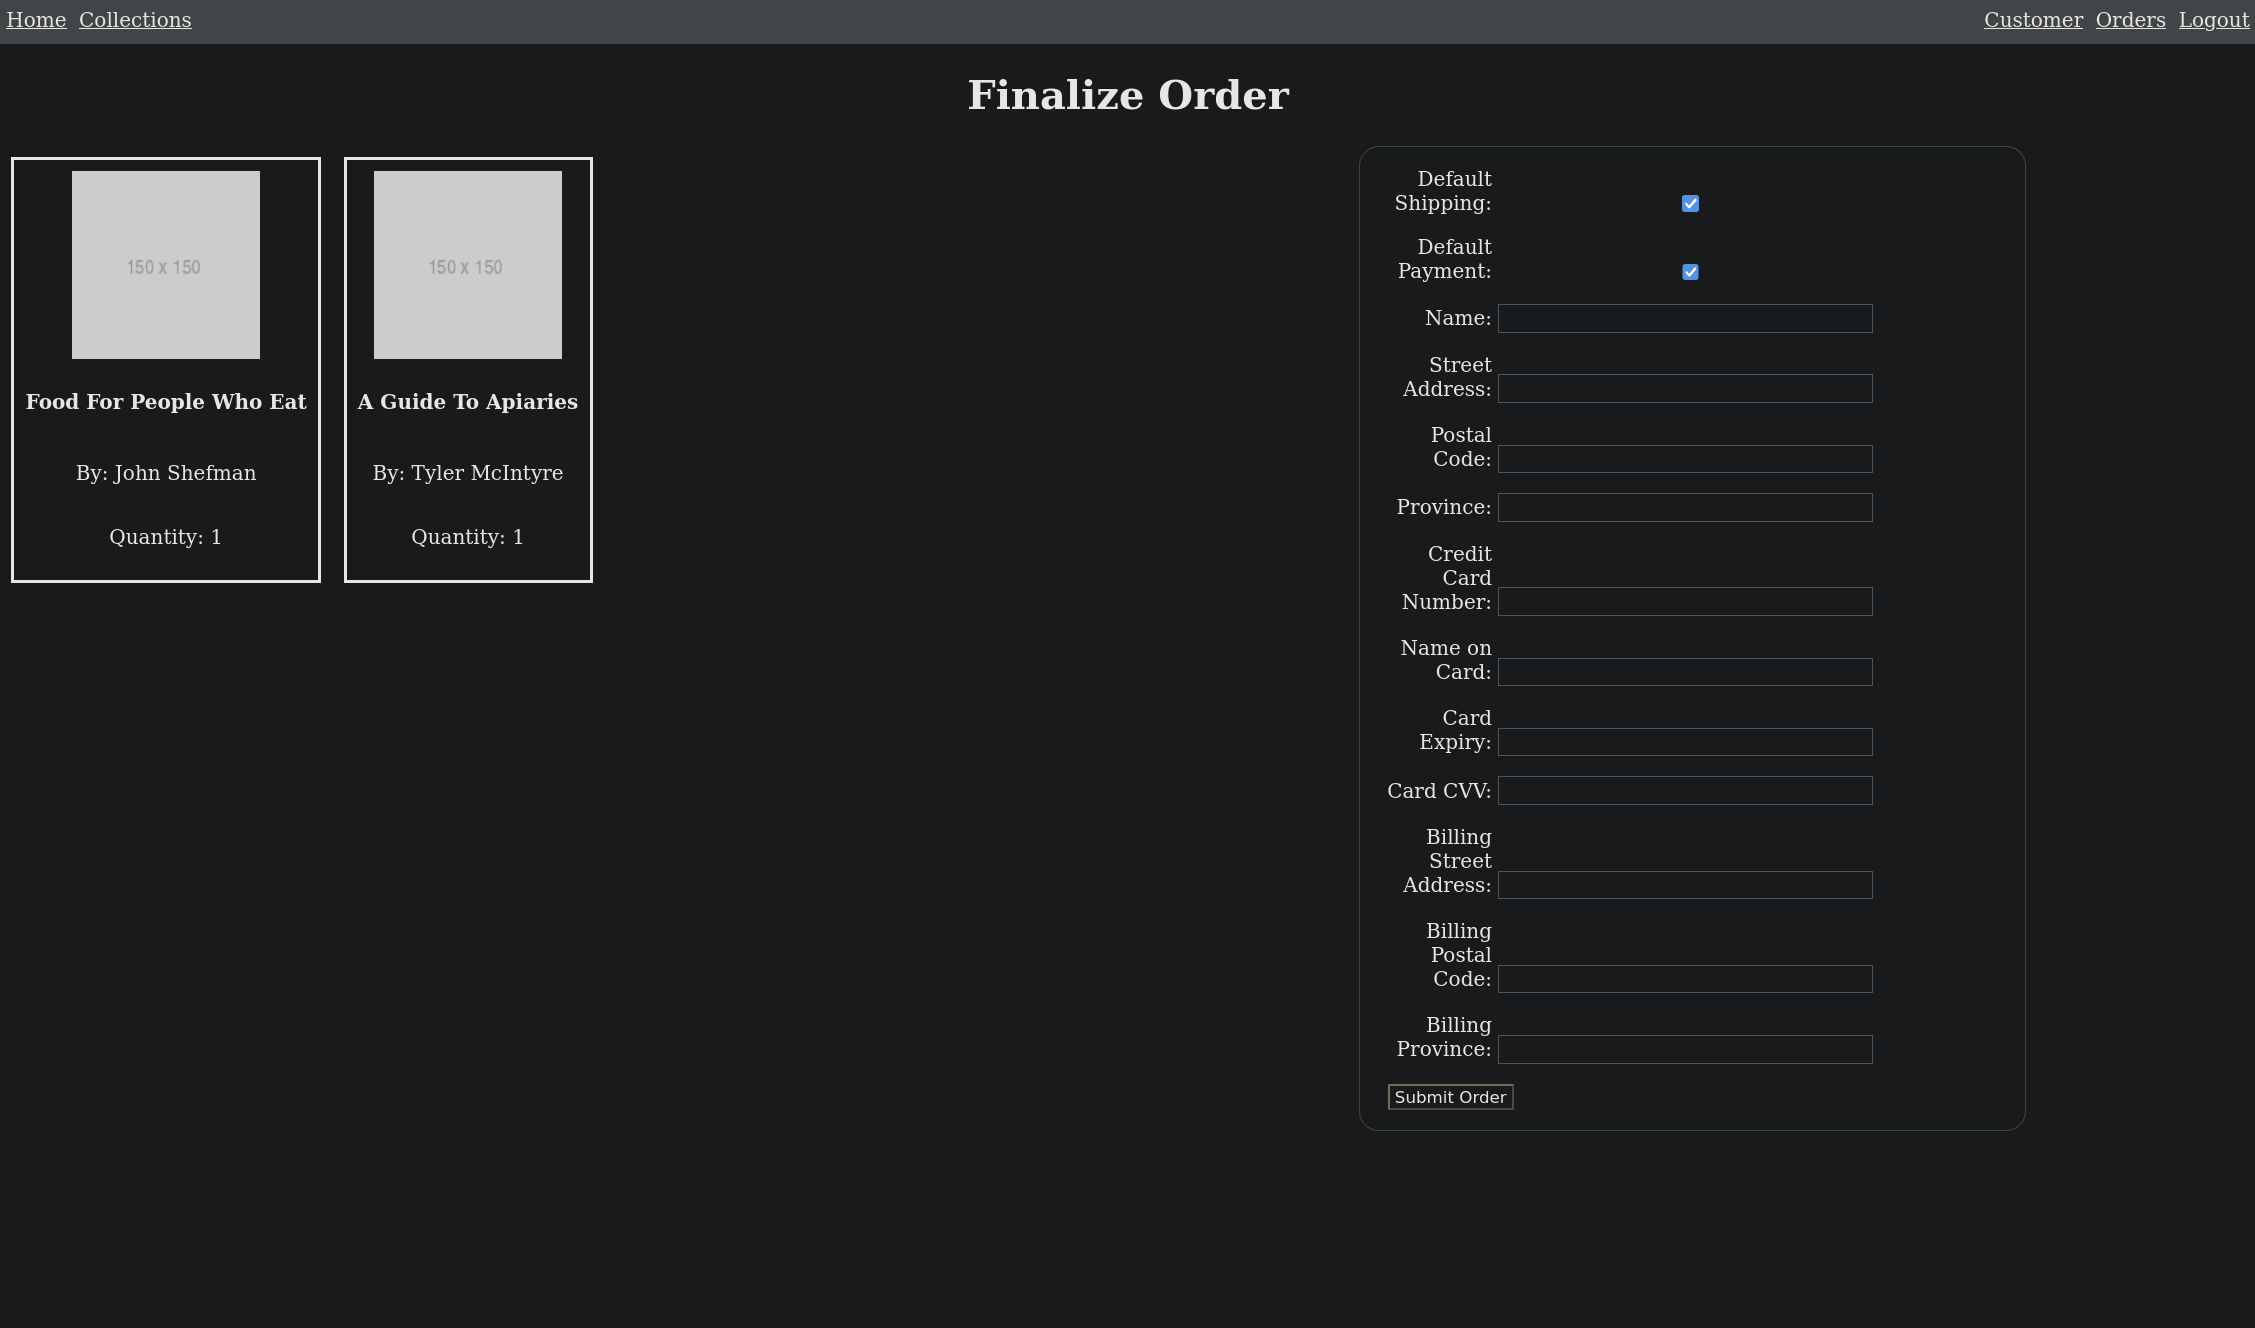
\includegraphics[width=\textwidth]{checkout}
  Create Book
  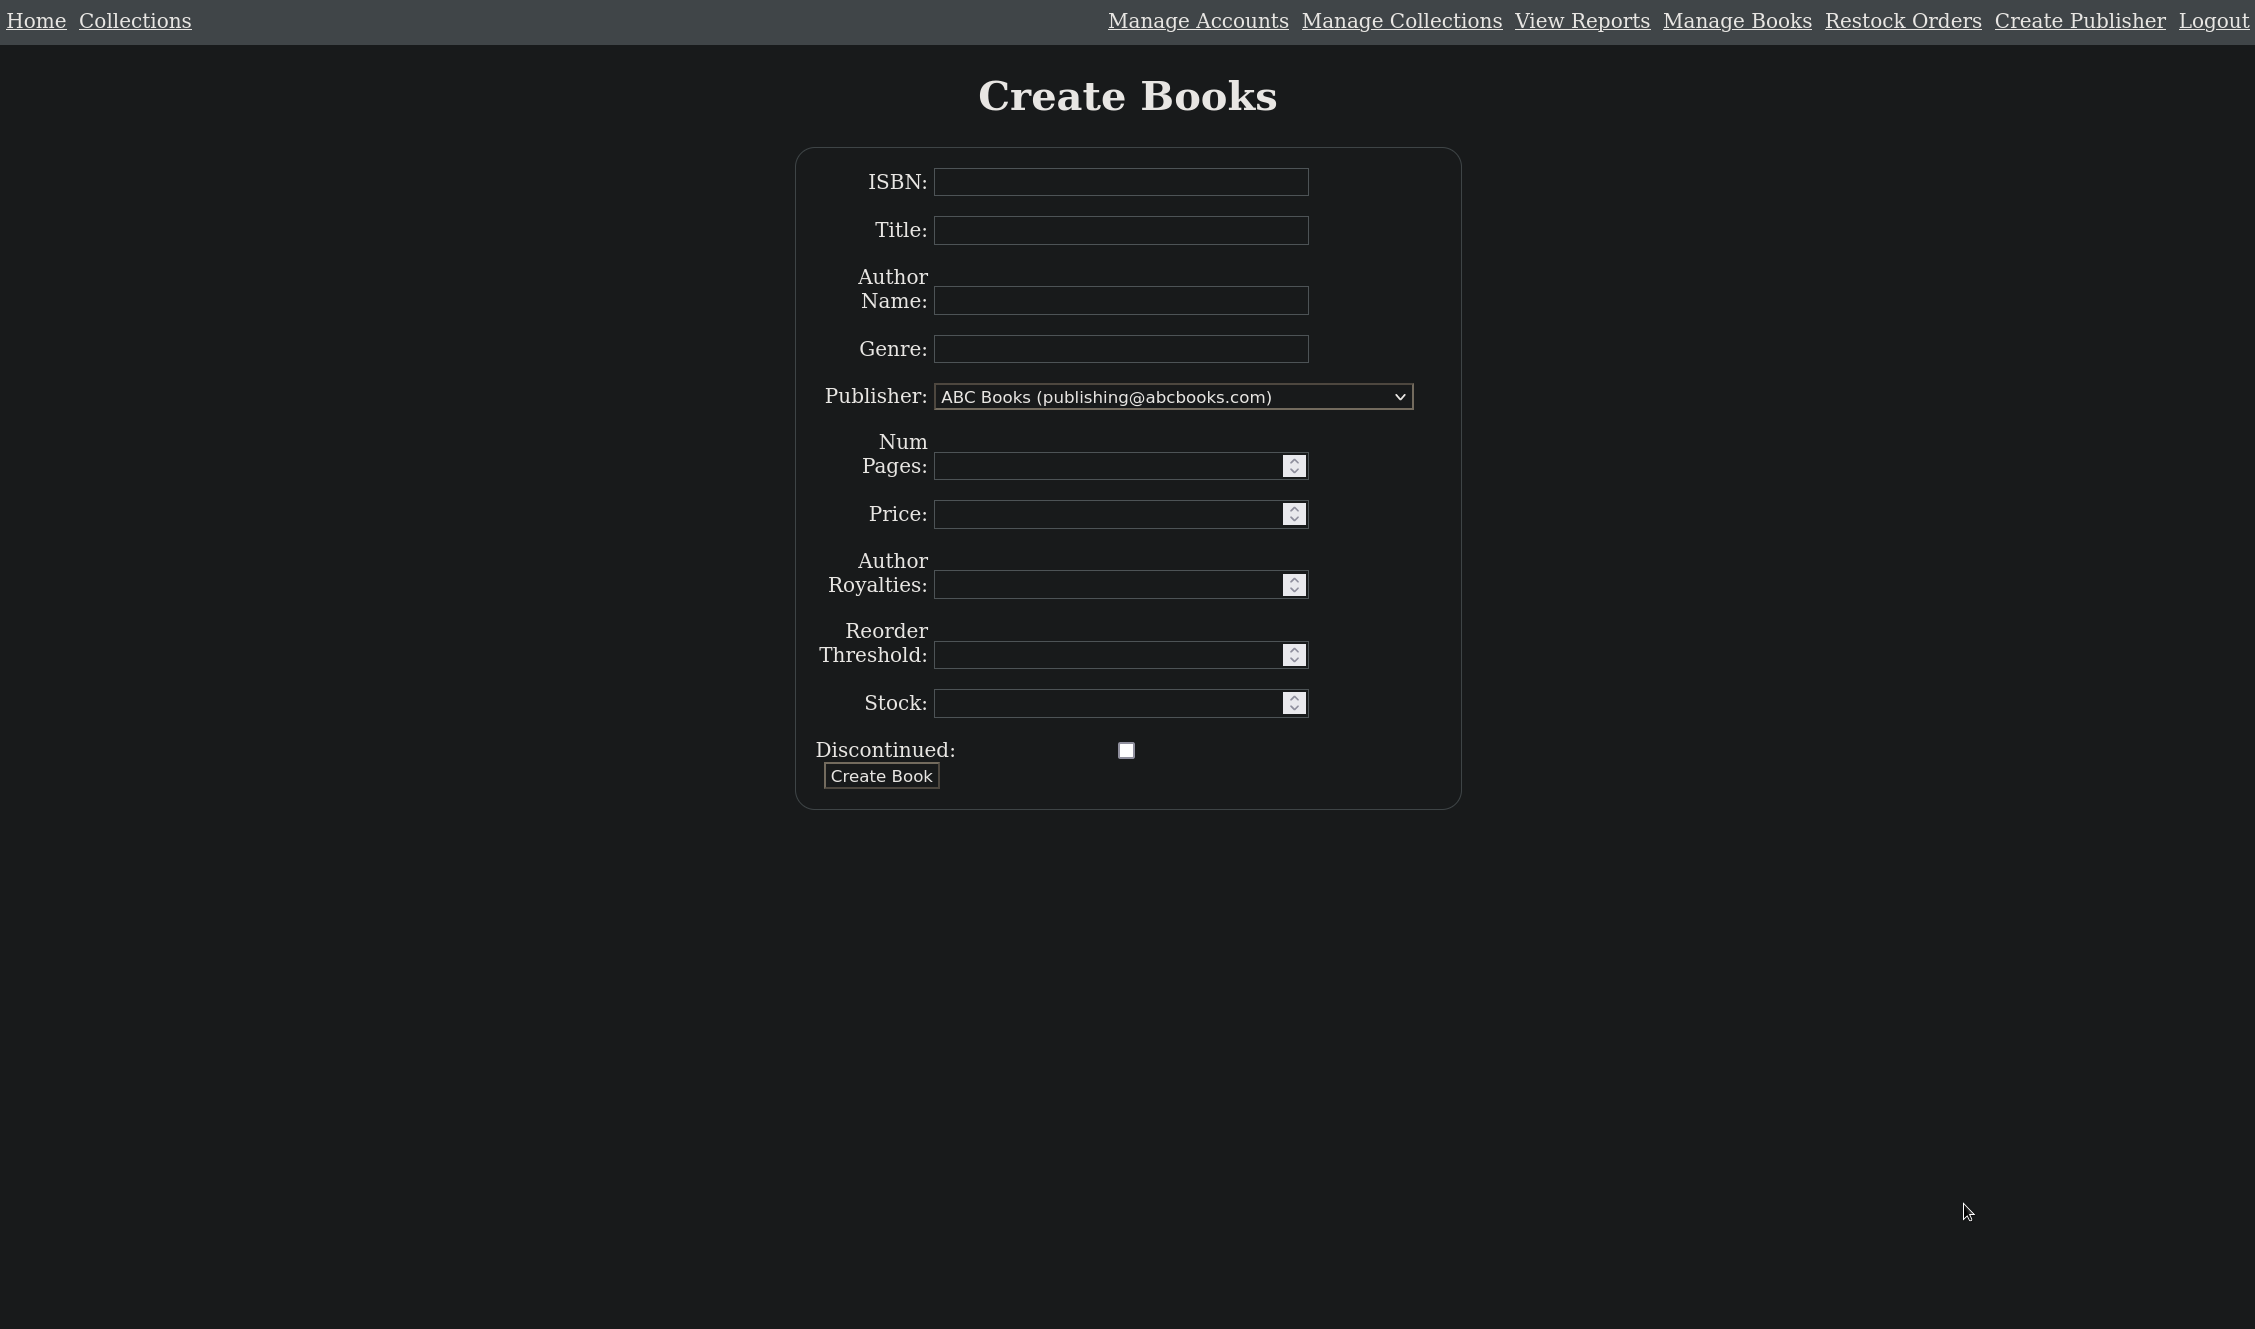
\includegraphics[width=\textwidth]{create_books}
\end{center}


\section{Bonus Features}
Some notable extra features are:
\begin{itemize}
  \item Password hashing and salting using the bcrypt algorithm for all logins (customers and owners)
  \item Encrypted cookies
  \item Type level access proofs (type level proofs that only owners can delete accounts, etc.) more details \href{https://rocket.rs/v0.4/guide/requests/#custom-guards}{here}.
  \item High performance and scalability courtesy of the Rust language
  \item Trivial usage by multiple users at the same time due to the web server nature and Rust's concurrency guaranteees
  \item Easy deployments to single nodes courtesy of the Rust toolchain
  \item Minimal use of javascript/client-side rendering for high performance and accessibility out of the box achieved through use of SSR and HTML templates
  \item String similarity search with titles using the sorensen dice algortithm provided by the strsim Rust crate
  \item Curated book collections by owners
\end{itemize}


\section{Github Repository}
The github for the project is \href{https://github.com/Eliasin/lookInnaBook}{here} (https://github.com/Eliasin/lookInnaBook). I have also deployed it to a DigitalOcean droplet for you to try out \href{http://owncloud.eliasin.ca:8000/}{here} (http://owncloud.eliasin.ca:8000/). (Note while creating accounts that while passwords are not stored because of the hashing, the site does not implement HTTPS and therefore passwords are sent across the internet unencrypted.)

\section{Appendix}
I am available on Dec 20th from 4 p.m. to 5 p.m.
\end{document}
